\documentclass[
  bibliography=totoc,     % Literatur im Inhaltsverzeichnis
  captions=tableheading,  % Tabellenüberschriften
  titlepage=firstiscover, % Titelseite ist Deckblatt
]{scrartcl}

% Paket float verbessern
\usepackage{scrhack}

% Warnung, falls nochmal kompiliert werden muss
\usepackage[aux]{rerunfilecheck}

% unverzichtbare Mathe-Befehle
\usepackage{amsmath}
% viele Mathe-Symbole
\usepackage{amssymb}
% Erweiterungen für amsmath
\usepackage{mathtools}

% Fonteinstellungen
\usepackage{fontspec}
% Latin Modern Fonts werden automatisch geladen
% Alternativ zum Beispiel:
%\setromanfont{Libertinus Serif}
%\setsansfont{Libertinus Sans}
%\setmonofont{Libertinus Mono}

% Wenn man andere Schriftarten gesetzt hat,
% sollte man das Seiten-Layout neu berechnen lassen
\recalctypearea{}

% deutsche Spracheinstellungen
\usepackage[main=ngerman]{babel}


\usepackage[
  math-style=ISO,    % ┐
  bold-style=ISO,    % │
  sans-style=italic, % │ ISO-Standard folgen
  nabla=upright,     % │
  partial=upright,   % ┘
  warnings-off={           % ┐
    mathtools-colon,       % │ unnötige Warnungen ausschalten
    mathtools-overbracket, % │
  },                       % ┘
]{unicode-math}

% traditionelle Fonts für Mathematik
\setmathfont{Latin Modern Math}
% Alternativ zum Beispiel:
%\setmathfont{Libertinus Math}

\setmathfont{XITS Math}[range={scr, bfscr}]
\setmathfont{XITS Math}[range={cal, bfcal}, StylisticSet=1]

% Zahlen und Einheiten
\usepackage[
  locale=DE,                   % deutsche Einstellungen
  separate-uncertainty=true,   % immer Fehler mit \pm
  per-mode=symbol-or-fraction, % / in inline math, fraction in display math
]{siunitx}

% chemische Formeln
\usepackage[
  version=4,
  math-greek=default, % ┐ mit unicode-math zusammenarbeiten
  text-greek=default, % ┘
]{mhchem}

% richtige Anführungszeichen
\usepackage[autostyle]{csquotes}

% schöne Brüche im Text
\usepackage{xfrac}

% Standardplatzierung für Floats einstellen
\usepackage{float}
\floatplacement{figure}{htbp}
\floatplacement{table}{htbp}

% Floats innerhalb einer Section halten
\usepackage[
  section, % Floats innerhalb der Section halten
  below,   % unterhalb der Section aber auf der selben Seite ist ok
]{placeins}

% Seite drehen für breite Tabellen: landscape Umgebung
\usepackage{pdflscape}

% Captions schöner machen.
\usepackage[
  labelfont=bf,        % Tabelle x: Abbildung y: ist jetzt fett
  font=small,          % Schrift etwas kleiner als Dokument
  width=0.9\textwidth, % maximale Breite einer Caption schmaler
]{caption}
% subfigure, subtable, subref
\usepackage{subcaption}

% Grafiken können eingebunden werden
\usepackage{graphicx}
% größere Variation von Dateinamen möglich
\usepackage{grffile}

% schöne Tabellen
\usepackage{booktabs}

% Verbesserungen am Schriftbild
\usepackage{microtype}

% Literaturverzeichnis
\usepackage[
  backend=biber,
]{biblatex}
% Quellendatenbank
\addbibresource{lit.bib}
\addbibresource{programme.bib}

% Hyperlinks im Dokument
\usepackage[
  german,
  unicode,        % Unicode in PDF-Attributen erlauben
  pdfusetitle,    % Titel, Autoren und Datum als PDF-Attribute
  pdfcreator={},  % ┐ PDF-Attribute säubern
  pdfproducer={}, % ┘
]{hyperref}
% erweiterte Bookmarks im PDF
\usepackage{bookmark}

% Trennung von Wörtern mit Strichen
\usepackage[shortcuts]{extdash}

\author{%
  Johannes Lamers\\%
  \href{mailto:johannes.lamers@edu.edu}{johannes.lamers@udo.edu}%
  \and%
  Sebastian Fischer\\%
  \href{mailto:sebastian.fischer@udo.edu}{sebastian.fischer@udo.edu}%
}
\publishers{TU Dortmund – Fakultät Physik}


\subject{803}
\title{Das Hooksche Gesetz}
\date{%
  Durchführung: 02.11.2019
  \hspace{3em}
  Abgabe: DATUM
}

\begin{document}

\maketitle
\thispagestyle{empty}
\tableofcontents
\newpage

\section{Theorie}
\label{sec:Theorie}
Analog zu der Masse bei der Translation lässt sich bei Rotationen das Trägheitsmoment definieren. Es wird dabei als Trägheit des Objektes gegenüber einer Rotation bezüglich einer Rotationsachse verstanden. Es lässt sich durch die Gleichung 
\begin{equation}
    I=\sum_{i}r_i^2\cdot m_i
\end{equation}
berechnen. $r_i$ ist dabei der Abstand des Massenelements $m_i$ zur Rotationsachse.
Für kontinuierliche Masseverteilungen kann zum berechnen des Trägheitsmoments die Gleichung
\begin{equation}
    I=\rho\int_V r_\perp^2 \,\symup{d}V
\end{equation}
verwendet werden. $\rho$ beschreibt die Dichte des Materials.


\begin{figure}
    \caption{Trägheitsmomente einiger Körper.}
    \centering
    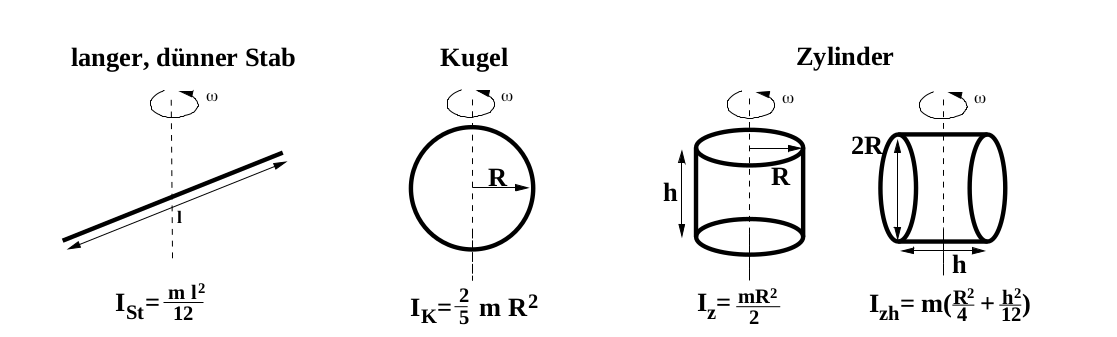
\includegraphics[height=4cm]{data/Probekoerper.png}
    \label{fig:probe}
\end{figure}


In Abbildung \ref{fig:probe} sind die in dem Versuch benötigten Trägheitsmomente aufgeführt. 
Falls die Rotationsachse um einen Abstand a zu einer parallelen Rotationsachse durch den Schwerpunkt verschoben ist, kann das Trägheitsmoment über die Gleichung
\begin{equation}
\label{eqn:stein}
    I=I_s+m\cdot a^2
\end{equation}
berechnet werden. Diese Gleichung wird auch 'Satz von Steiner' gennant.  $I_s$ ist das Trägheitsmoment bezüglich der Rotationsachse durch den Schwerpunkt.


Bei diesem Versuch wirkt bei einer Drehung um den Winkel $\phi$ durch eine Torsionsfeder ein rücktreibendes Drehmoment auf das Objekt. So führt das System beim loslassen eine Schwingung um die Drehachse durch. Die Schwingungsdauer lässt sich dann über 
\begin{equation}
\label{eqn:T}
    T=2\pi \sqrt{\frac{I}{D}}
\end{equation}
berechnen. $D$ entspricht der Winkelrichtgröße, welche über  
\begin{equation}
\label{eqn:M}
    M=D\cdot \phi
\end{equation}
mit dem Drehmoment in Zusammenhang steht.
Damit die Schwingung in einem harmonischen Bereich abläuft, ist $\phi$ auf kleine Auslenkungen beschränkt.


Das Volumen eines Zylinders wird über die Gleichung
\begin{equation}
    \label{eqn:Z}
    V=\frac{d^2}{4}\pi h
\end{equation}
bestimmt. Dabei ist $d$ der Durchmesser und $h$ die Höhe des Zylinders.

%In knapper Form sind die physikalischen Grundlagen des Versuches, des Messverfahrens, sowie sämtliche für die Auswertung erforderlichen Gleichungen darzustellen. (Keine Herleitung)

%(eventuell die Aufgaben)

%Der Versuchsaufbau: Beschreibung des Versuchs und der Funktionsweise (mit Skizze/Bild/Foto)


    \section{Aufbau}
    \label{sec:Aufbau}

    Eine Feder wird senkrecht mit einem stationären Newtonmeter verbunden, sodass beim Auslenken
    der Feder das Newtonmeter die rücktreibende Kraft anzeigen kann. Die Feder wird mit einem 
    Faden verbunden, welcher über eine Umlenkrolle enlang eines waagerecht angebrachten Lineals verläuft.
    Mit Hilfe einer Klemme kann der Faden an einer jeweiligen Position an das Lineal fixiert werden.
    Die Feder sollte in Ruhe hängen, wenn sich die Klemme auf der 0 des Lineals befindet und der Faden sollte 
    dauerhaft auf Spannung sein.

\section{Durchführung}
\label{sec:Durchführung}

\subsection{Justierung} 
\label{sub:Justierung}


Vor Beginn des eigentlichen Versuchs müssen vorbereitende Justierungen durchgeführt werden. Beide Schwingkreise müssen 
auf die gleiche Resonanzfrequenz eingestellt werden.
Dabei wird, wie in Bild \ref{fig:bild5} dargestellt, eine variierbare Kapazität in einen der Schwingkreise geschaltet. Über ein
Oszilloskop im XY-Betrieb können Lissajous-Figuren dargestellt werden. Zuerst wird dabei eine ungefähre Ermittllung der Resonanzfrequenz vorgenommen, in dem der X-Eigang von der 
Generatorspannung getrennt wird. Durch Veränderung der Frequenz sollen die beobachtbaren Lissajous-Figuren verschwinden. Ist das der Fall, so sind Strom und Spannung in Phase. In der Praxis gestalltet sich das auf Grund von unzureichend genauen Justiermöglichkeiten relativ schwierig.
Durch eine möglichst gute Minimierung der von der Figur berandeten Fläche kann
ebenfalls in guter Näherung die Resonanzfrequenz gefunden werden. Die Schaltung wird wieder wie in Abbildung \ref{fig:bild5} aufgebaut. Daraufhin gilt es den verstellbaren Kondensator so zu justieren, sodass auch der zweite Schwingkreis auf die eben gefundene Frequenz eingestellt wird.


\begin{figure}

    \centering
    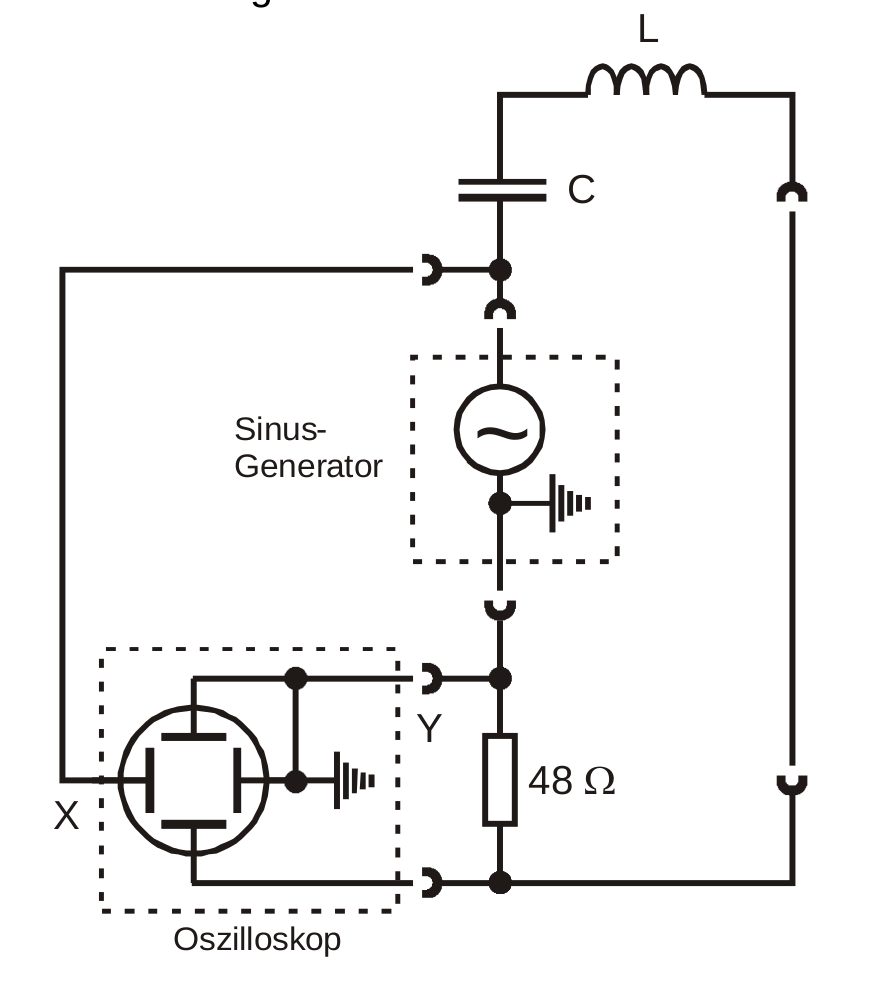
\includegraphics[height=6.0cm]{data/Bild5.png}
    \caption{Schaltbild zur Bestimmung der Resonanzfrequenz eines Schwingkreises.}
    \label{fig:bild5}
\end{figure}

\subsection{Untersuchung einer Schwebung} 
\label{sub:Untersuchung einer Schwebung}



Der Versuch soll mit Hilfe von Schwebungen den Energieaustausch zwischen den beiden Schwingkreisen darstellen.
Dafür wird die Schaltung nach Abbildung \ref{fig:bild6} aufgebaut. Es ist zu Beachtem, dass nur der linke Schwingkreis durch einen Sinusgenerator angeregt wird.
Mit Hilfe eines Oszilloskops können bei Variation des 
Kondensators $C_K$ verschiedene Schwebungen beobachtet werden. Die Kapazität wird dabei bei von $2\si{\nano\farad}$  bis $12\si{\nano\farad}$
schrittweise erhöht. Jedesmal wird anschließend das Verhältnis der beiden Frequenzen ermittelt, indem die Anzahl der Schwingungsmaxima innerhalb einer Schwebungsperiode 
gezählt werden.


\subsection{Bestimmung der Fundamentalschwingungen}
\label{sub:Bestimmung der Fundamentalschwingungen}



Der zweite Teil des Versuchs zielt auf des ermitteln der Fundamentalschwingungen ab. Die Schaltung wird, bis auf das ersetzten des Rechteckgenerators in
einen Sinusgenerator, so wie in Abbildung \ref{fig:bild6} beibehalten. Die Generatorspannung soll dabei auf den X-Eingang gegeben werden.
Durch erneute Einstellung des XY-Betriebes können wieder Lissajous-Figuren beobachtet werden. Der Kondensator $C_K$ wird wieder schrittweise verändert und jedesmal die Frequenzen ermittelt, bei 
denen die Lissajous-Figur verschwindet. 


\begin{figure}

    \centering
    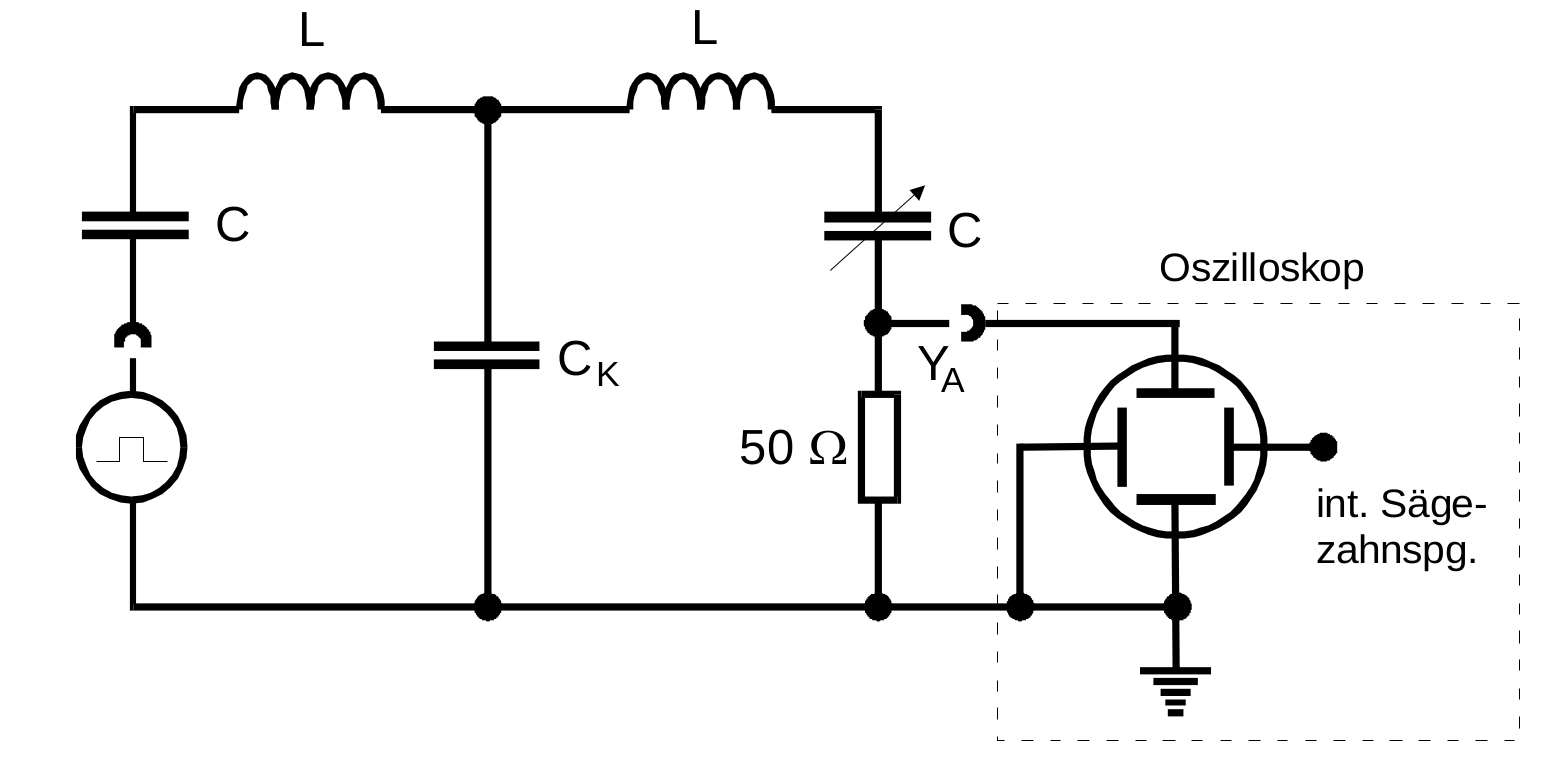
\includegraphics[height=6.0cm]{data/Bild6.png}
    \caption{Schaltbild zur Bestimmung der Fundamentalschwingungen eines gekoppelten Systems.}
    \label{fig:bild6}
\end{figure}





%Was wurde gemessen bzw. welche Größen wurden variiert?
\section{Auswertung}
\label{sec:Auswertung}


\subsection{Statische Methode}
In den folgenden Plots werden jeweils zwei Temperaturverläufe verglichen. Im Plot\ref{fig:t1t4} wird der breite und der schmale 
Messingstab untersucht, in Plot\ref{fig:t5t8} werden Aluminium und Edelstahl auf ihre Temperaturen untersucht. Die Temperaturen werden hier jeweils
an den vom Thermoelement weiter entfernten Thermometern gemessen.

\begin{figure}
    \centering
    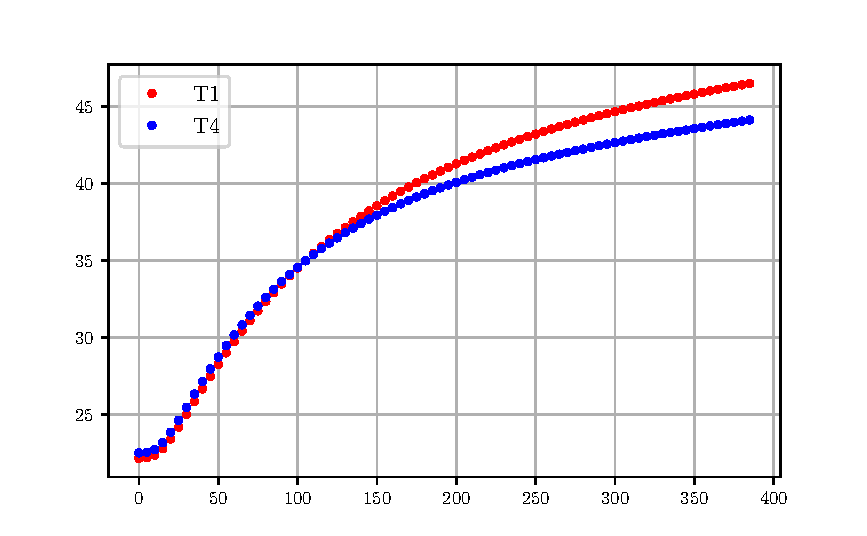
\includegraphics[width=\textwidth]{data/T1T4.pdf}
    \caption{Temperaturverläufe der Messingstäbe}
    \label{fig:t1t4}
\end{figure}

\begin{figure}
    \centering
    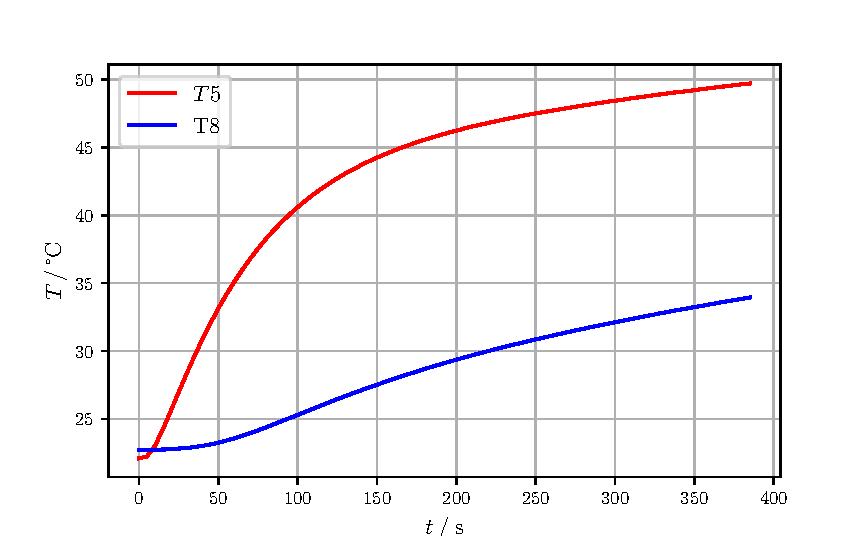
\includegraphics[width=\textwidth]{data/T5T8.pdf}
    \caption{Temperaturverläufe von Aluminium und Edelstahl}
    \label{fig:t5t8}
\end{figure}

In der Auflistung stehen die in den Plots gezeigten Temperaturen zu Ende der statischen Messung:
\begin{align*}
T_1(t=385) =& 46.50 \si{\celsius}\\
T_4(t=385) =& 44.13 \si{\celsius}\\
T_5(t=385) =& 49.71 \si{\celsius}\\
T_8(t=385) =& 33.94 \si{\celsius}
\end{align*}

%Es ist zu sehen, dass die Temperatur des Aluminiumstabes am höchsten ist. Da alle Thermometer den gleichen Abstand
%zum Heizkörper haben und deren anfängliche Temperaturen bis auf geringe Abweichungen gleich sind, kann daraus 
%geschlossen werden, dass Aluminium die höchste Wärmeleitfähigkeit hat.

Zur Berechnung des Wärmestroms wird die Querschnittsfläche $A$ der einzelnen Stäbe aus der Versuchsanleitung entnommen.
Die Wärmeleitfähigkeiten $\kappa$ sind aus der Literatur\cite{V204} übernommen und die Entfernung $\Delta x$ der jeweiligen $T$ 
werden abgemessen.

\begin{align*}
\kappa _\text{Messing}& = 109\si{\watt\per\meter\kelvin} \\
A_\text{Messing,breit}& = 48\cdot 10^{-6}\si{\meter\squared} \\
\Delta x_\text{Messing,breit}& = 0,03\si{\meter} \\
\kappa _\text{Edelstahl}& = 16\si{\watt\per\meter\kelvin} \\
A_\text{Edelstahl}& = 48\cdot 10^{-6}\si{\meter\squared} \\
\Delta x_\text{Edelstahl}& = 0,03\si{\meter} 
\end{align*}

\begin{table}
    \centering
    \caption{Wäremestrom von Messing und Edelstahl}
    \label{tab:deltaq}
    \begin{tabular}{S S S S S}
        \toprule
        {$t\:/\:\si{s}$} & {$\Delta T_{21}\:/\:\si{\kelvin}$} & {$\frac{\text{d}Q_{21}}{\text{d}t}\:/\:\si{\watt}$} & 
        {$\Delta T_{78}\:/\:\si{\kelvin}$} & {$\frac{\text{d}Q_{78}}{\text{d}t}\:/\:\si{\watt}$} \\
        \midrule
        75 & 7.11 & 1.23998 & 12.65 & 0.32384 \\
        150 & 4.80 & 0.83712 & 13.52 & 0.34611 \\
        225 & 3.55 & 0.61912 & 12.57 & 0.32179 \\
        300 & 2.93 & 0.51099 & 11.77 & 0.30131 \\
        375 & 2.61 & 0.45518 & 11.21 & 0.28698 \\
        \bottomrule 
    \end{tabular}
\end{table}
Der folgende Plot vergleicht die Temperaturunterschiede der nahen und fernen Thermometer des jeweils gleichen Stabs. Dieser 
Temperaturunterschied ist hier für Messing und Edelstahl gezeigt.

\begin{figure}
    \centering
    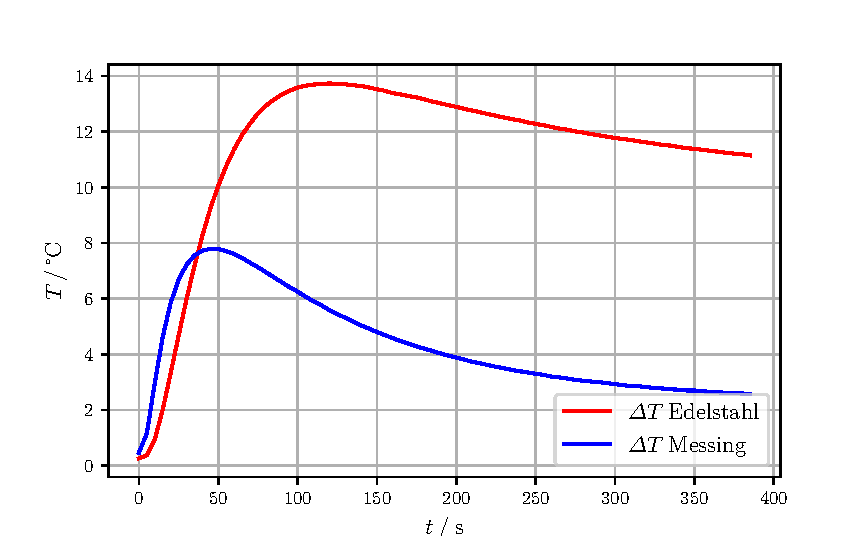
\includegraphics[width=\textwidth]{data/deltaT.pdf}
    \caption{Temperaturunterschied innerhalb eines Stabes für Messing und Edelstahl}
    \label{fig:deltat}
\end{figure}


\subsection{Dynamische Methode}

Im Folgenden wird anhand der Temperaturamplituden $A_i$ und der Phasendifferenzen $\Delta t$ die Wärmeleitfähigkeit $\kappa$
der verschiedenen Metalle berechnet. Für Messing und Aluminium wird dafür die Messung mit 80$\si{\s}$ Periodendauer 
und für Edelstahl die Messung mit 200$\si{\s}$ Periodendauer verwendet.
Die Amplituden, sowie die Phasendifferenzen können aus den Messwerten abgelesen werden. Damit kann nach Gleichung\ref{eqn:kappa}
jeweils $\kappa$ berechnet werden.

\begin{table}
    \centering
    \caption{Amplituden und Phasendifferenz der Temperaturverläufe von Messing}
    \label{tab:amp_m}
    \begin{tabular}{S S S}
        \toprule
        {$A_1\:/\:\si{\kelvin}$} & {$A_2\:/\:\si{\kelvin}$} & {$\Delta t\:/\:\si{\s}$} \\
        \midrule
        4.585 & 12.890 & 16 \\
        4.245 & 12.705 & 14 \\
        4.070 & 12.555 & 13 \\
        \bottomrule
    \end{tabular}
\end{table}

\begin{figure}
    \centering
    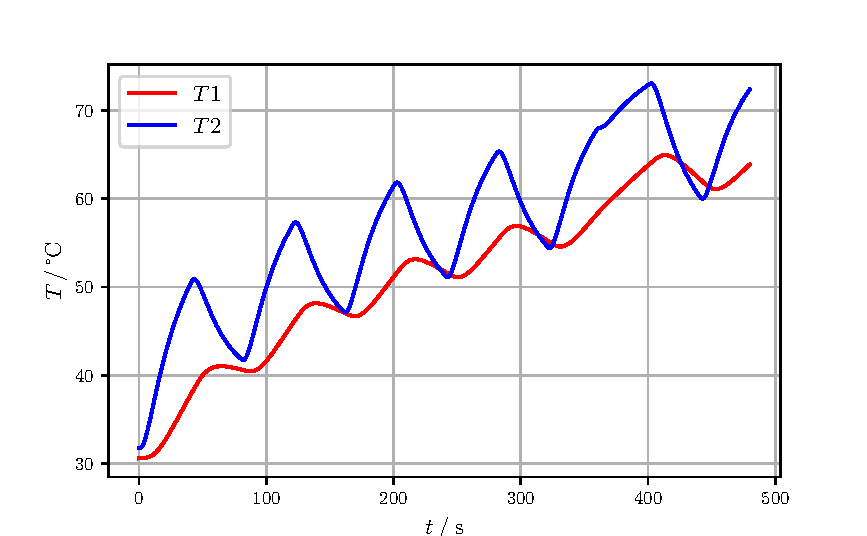
\includegraphics[width=\textwidth]{data/T1T2.pdf}
    \caption{Temperaturunterschied innerhalb des Messingstabes}
    \label{fig:t1t2}
\end{figure}

Die Konstanten für Messing sind:
\begin{align*}
    \rho& = 8520\:\si{\kilo\gram\per\meter\cubed} \\
    c& = 385\:\si{\joule\per\kilo\gram\kelvin}
\end{align*}

Daraus ergibt sich mit der Gleichung\ref{eqn:kappa} für die Wärmeleitfähigkeit:
\begin{equation*}
    \kappa_{\text{Messing}} = \SI{95(7)}{\watt\per\meter\kelvin}
\end{equation*}   

\begin{table}
    \centering
    \caption{Amplituden und Phasendifferenz der Temperaturverläufe von Aluminium}
    \label{tab:amp_a}
    \begin{tabular}{S S S}
        \toprule
        {$A_5\:/\:\si{\kelvin}$} & {$A_6\:/\:\si{\kelvin}$} & {$\Delta t\:/\:\si{\s}$} \\
        \midrule
        8.060 & 15.955 & 8 \\
        7.635 & 15.600 & 7 \\
        7.500 & 15.515 & 7 \\
        \bottomrule
    \end{tabular}
\end{table}

\begin{figure}
    \centering
    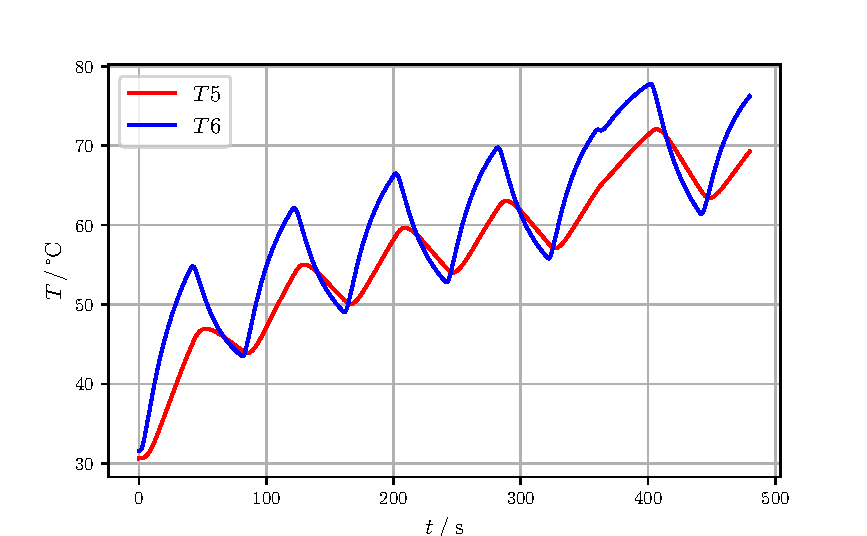
\includegraphics[width=\textwidth]{data/T5T6.pdf}
    \caption{Temperaturunterschied innerhalb des Aluminiumstabes}
    \label{fig:t5t6}
\end{figure}

Die Konstanten für Aluminium sind:
\begin{align*}
    \rho& = 2800\:\si{\kilo\gram\per\meter\cubed} \\
    c& = 850\:\si{\joule\per\kilo\gram\kelvin}
\end{align*}

Daraus ergibt sich für die Wärmeleitfähigkeit:
\begin{equation*}
    \kappa_{\text{Aluminium}} = \SI{202(11)}{\watt\per\meter\kelvin}
\end{equation*}

\begin{table}
    \centering
    \caption{Amplituden und Phasendifferenz der Temperaturverläufe von Edelstahl}
    \label{tab:amp_e}
    \begin{tabular}{S S S }
        \toprule
        {$A_7\:/\:\si{\kelvin}$} & {$A_8\:/\:\si{\kelvin}$} & {$\Delta t\:/\:\si{\s}$} \\
        \midrule
        19.575 & 3.110 & 66 \\
        19.410 & 2.920 & 60 \\
        19.515 & 2.955 & 46 \\
        19.040 & 2.610 & 51 \\
        \bottomrule
    \end{tabular}
\end{table}

\begin{figure}
    \centering
    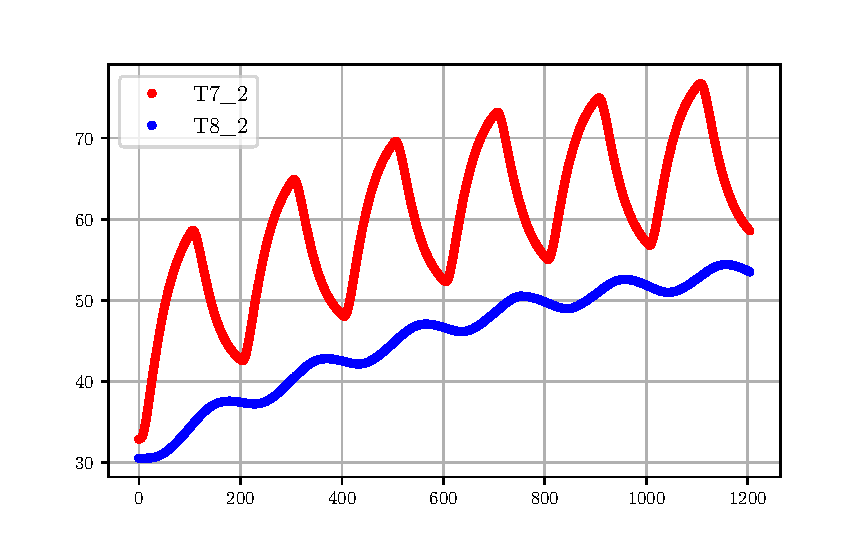
\includegraphics[width=\textwidth]{data/T7T8.pdf}
    \caption{Temperaturunterschied innerhalb des Edelstahlstabes}
    \label{fig:t7t8}
\end{figure}

Die konstanten für Edelstahl sind:
\begin{align*}
    \rho& = 8000\:\si{\kilo\gram\per\meter\cubed} \\
    c& = 400\:\si{\joule\per\kilo\gram\kelvin}
\end{align*}

Daraus ergibt sich für die Wärmeleitfähigkeit:
\begin{equation*}
    \kappa = \SI{13.6(11)}{\watt\per\meter\kelvin}
\end{equation*}

\section{Diskussion}
\label{sec:Diskussion}

Grundsätzlich fällt auf, dass bei allen über die Messwerte berechneten Größen
eine relativ große Standardabweichung zu sehen ist. Bei der Wheaton Brücke liegt diese
beispielsweise bei etwa 10\%. Dies ist auch die Größenordnung für die restlichen Teilversuche,
wobei manche Größen, wie z.B. die durch die Kapazitätsmessbrücke errechnete Kapazität $C_x$,
sogar eine Standardabweichung von über 30\% haben. Allgemein sind alle hier zu bestimmenden
Werte sehr ungenau. Ein Bauteil, dessen Wert hier berechnet wurde, wäre äußerst unpraktikabel,
in einem neuen Versuchsaufbau zu verwenden, da der dann zu messende Wert durch die hohen Standardabweichungen
des Bauteils deutlich an Präzision verlieren würde. 

In jeder der Brückenschaltungen wurde, unabhänging vom speziellen Aufbau, das Potentiometer $\frac{R_3}{R_4}$,
der selbe Oszillograph und der selbe Generator verwendet. Da auffällig ist, dass bei allen Versuchen die Abweichungen
sehr groß sind, wäre es vorstellbar, dass eines der eben aufgezählten Bauteile beschädigt ist. Das Netzteil scheint an 
dieser Stelle nicht der dafür verantwortliche Faktor zu sein, da die davon ausgehende Speisespannung $U_S$ zwischendurch 
gemessen wurde und jedes Mal der eingestellten Spannung von 2,5\si{\volt} entsprach. Um dem Ursprung des Fehlers genauer 
ausmachen zu können, liegen hier nicht genug Informationen vor, ein oder mehrere defekte oder ungenaue Komponetenten in 
den jeweiligen Aufbauten sind daher die Annahme.

Bei der Auswertung der Wien-Robinson-Brücke \ref{fig:wien} ist beim Vergleich der Messwerte mit der Theoriekurve zu sehen,
dass die Werte in der Nähe des Minimums relativ gut mit der Theorie übereinstimmen. Das gemessene Minimum weicht hier recht stark
von null ab, was unter anderem daran liegen könnte, dass in dieser Umgebung die Messwerte nicht kleinschrittig genug aufgenommen 
wurden, und somit das optimal messbare Minimum übersprungen wurde. Damit wurde auch die Klirrfaktorbestimmung ungenau. Außerdem wurde beim Bestimmen 
des Klirrfaktors nur eine Oberwelle einbezogen, wodurch ebenfalls eine gewisse Ungenauigkeit entsteht.
Bei einer höheren Anzahl an Messwerten in der Nähe des Minimums hätte eine genauere, und wahrscheinlich etwas niedrigere Minimalfreqenz
ermittelt werden können, wodurch der Klirrfaktor ebenfalls niedriger ausfallen würde.  Es fällt außerdem auf, dass Messwerte ab einem bestimmten 
Punkt rechts vom Minimum wieder abfallen, obwohl sie laut Theorie konstant bleiben müssten. Dies könnte an den Streukapazitäten der Bauteile und des Oszillographen liegen, 
welche besonders bei hohen Frequenzen an Gewicht erhalten.

%Kurze Zusammenfassung der Ergebnisse
%-Vergleich mit Literaturwerten
%-Vergleich mit verschiedenen Messverfahren
%-bei Abweichungen mögliche Ursachen finden

\printbibliography{}

\end{document}
